\documentclass[12pt]{article}

\usepackage{booktabs}% http://ctan.org/pkg/booktabs
\usepackage[utf8]{inputenc}
\usepackage{changepage}
\usepackage{pgfplots}
\usepackage{amssymb}
\usepackage{xcolor}
\usepackage{hyperref}
\usepackage{listings}
\usepackage[T1]{fontenc}
\usepackage[utf8]{inputenc}
\usepackage{adjustbox}
\usepackage{amsmath}
\usepackage{mathtools}
\usepackage{biblatex}
\lstset{
  language=Python,
  numbers=left,
  numberstyle=\tiny,
  stepnumber=1,
  numbersep=5pt,
  tabsize=4,
  basicstyle=\ttfamily,
  columns=fullflexible,
  keepspaces,
}
\hypersetup{
    colorlinks,
    citecolor=black,
    filecolor=black,
    linkcolor=black,
    urlcolor=black
}

% Set page size and margins
% Replace `letterpaper' with `a4paper' for UK/EU standard size
\usepackage[letterpaper,top=2cm,bottom=2cm,left=3cm,right=3cm,marginparwidth=1.75cm]{geometry}

% Useful packages
\usepackage{amsmath}
\usepackage{mathtools}
\usepackage{graphicx}
\newenvironment{para}{\begin{adjustwidth}{13mm}{}}{\end{adjustwidth}}

\newcommand\tab[1][1cm]{\hspace*{#1}}

\newcommand{\tabitem}{\llap{\textbullet}}
\newcommand{\Hsquare}{%
\text{\fboxsep=-.2pt\fbox{\rule{0pt}{1ex}\rule{1ex}{0pt}}}%
}

\newtheorem{Definizione}{Definizione}[subsection]
\newtheorem{Lemma}{Lemma}[subsection]
\newtheorem{Teorema/Definizione}{Teorema/Definizione}[subsection]
\newtheorem{Corollario}{Corollario}[subsection]
\newtheorem{Teorema}{Teorema}[subsection]
\newtheorem{Proposizione}{Proposizione}[subsection]
\newtheorem{Notazione}{Notazione}[subsection]
\newtheorem{Commento}{Commento}[subsection]
\newtheorem{Dimostrazione}{Dimostrazione}[subsection]
\newtheorem{Osservazione}{Osservazione}[subsection]
\newtheorem{Nota}{Nota}[subsection]

\title{Basi di dati}
\author{spitfire}
\date{A.A. 2023-2024}
\begin{document}
\begin{figure}
    \centering
    
\includegraphics[width=0.35\textwidth]{Images/Logo scienze bicocca.png}
\end{figure}

\vspace{10cm}
\date{A.A. 2023-2024}


\maketitle

\newpage

\tableofcontents
\newpage
\section{Introduzione}
Una base di dati è un \textbf{insieme organizzato di dati} utilizzati per il supporto allo svolgimento di attività (di un ente, azienda, ufficio, persona).
Facciamo un passo indietro e ricordiamo cos'è invece \textbf{l'informatica}:
essa è la \textbf{scienza del trattamento razionale dell'informazione}, spesso per mezzo di \textbf{macchine automatiche}.
Essa è considerata come supporto alla conoscenza umana e alla comunicazione.
L'informatica ha due anime:
\begin{itemize}
    \item \textbf{Metodologica}: i metodi per la soluzione di problemi e la gestione delle informazioni
    \item \textbf{Tecnologica}: i calcolatori elettronici e i sistemi che li utilizzano
\end{itemize}
\subsection{Sistemi informativi}
Un \textbf{sistema informativo} è un componente (sottosistema) di un'organizzazione che gestisce le informazioni di interesse (cioè utilizzate per il perseguimento degli scopi dell'organizzazione).
Le funzioni di un sistema informativo sono:
\begin{itemize}
    \item \textbf{Acquisizione/memorizzazione}
    \item \textbf{Aggiornamento}
    \item \textbf{Interrogazione}
    \item \textbf{Elaborazione}
\end{itemize}
Il concetto di "sistema informativo" è \textbf{indipendente da qualsiasi automazione}: esistono organizzazioni
la cui ragion d'essere è la \textbf{gestione di informazioni} (es. servizi anagrafici e banche) e che operano da secoli.
Anche prima di essere automatizzati, molti sistemi informativi si sono evoluti verso una \textbf{razionalizzazione e standardizzazione} delle procedure e dell'organizzazione delle informazioni.
\subsection{Sistema informatico}
Un \textbf{sistema informatico} è una porzione \textbf{automatizzata} di un sistema informativo; cioè la parte del sistema informativo che gestisce le informazioni con tecnologia informatica.
\begin{center}
    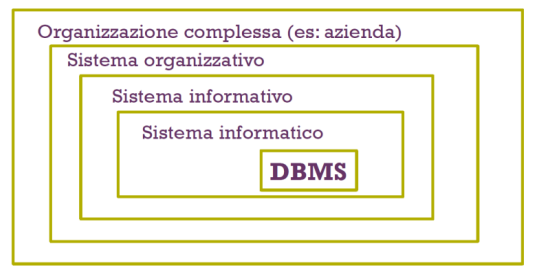
\includegraphics[width = 0.55\textwidth]{Images/1.PNG}
\end{center}
\newpage
\noindent
Un sistema informatico:
\begin{itemize}
    \item Garantisce che i dati siano conservati in modo \textbf{permanente} sui dispositivi di memorizzazione
    \item Permette un \textbf{rapido aggiornamento} dei dati per riflettere rapidamente le loro variazioni
    \item Rende i dati \textbf{accessibili alle interrogazioni} degli utenti
    \item Può essere \textbf{distribuito sul territorio}
\end{itemize}
\subsection{Gestione delle informazioni}
Nelle attività umane, le informazioni vengono gestite (registrate e scambiate) in forme diverse:
\begin{itemize}
    \item \textbf{Idee informali}
    \item \textbf{Linguaggio naturale} (scritto o parlato, formale o colloquiale, in una lingua o in un'altra)
    \item \textbf{Disegni, grafici e schemi}
    \item \textbf{Numeri e codici}
\end{itemize}
E su vari supporti, come la memoria umana, su carta o su dispositivi elettronici.
Nelle attività standardizzate dei sistemi informativi complessi, sono state introdotte col tempo forme di organizzazione e codifica delle informazioni via via più precise (e in un certo senso artificiali).
Ad esempio, nei servizi anagrafici si è iniziato con registrazioni discorsive per poi evolversi in registrazioni più complete.
\subsection{Informazioni e dati}
Nei sistemi informatici (e non solo), le \textbf{informazioni} vengono rappresentate in modo essenziale, spartano: attraverso i \textbf{dati}.
Diamo delle definizioni semantiche:
\begin{itemize}
    \item \textbf{Informazione}: notizia, dato o elemento che consente di avere conoscenza più o meno esatta di fatti, situazioni, modi di essere.
    \item \textbf{Dato}: ciò che è immediatamente presente alla conoscenza, prima di ogni elaborazione; (in informatica) elementi di informazione costituiti da simboli che debbono essere elaborati
\end{itemize}
I dati quindi hanno bisogno di essere interpretati!
\subsubsection{Perché i dati?}
La rappresentazione precisa di forme più ricche di informazione e conoscenza è difficile.
I dati costituiscono spesso una risorsa strategica, perché più stabili nel tempo di altri componenti (processi, tecnologie, ruoli, umani).
I dati rimangono gli stessi nella \textbf{migrazione} da un sistema al successivo.
\subsection{Basi di Dati e introduzione ai Database Management Systems (DBMS)}
Come già detto, una \textbf{base di dati} (DB) è una collezione di dati utilizzati per rappresentare le informazioni di interesse in un sistema informativo.
Un \textbf{Database Management System} (DBMS) è invece un \textbf{sistema software} capace di gestire collezioni di dati che siano \textit{grandi, condivise e persistenti}, assicurando la loro \textit{affidabilità e privatezza}.
Possiamo quindi dare due accezioni al termine \textbf{base di dati}:
\begin{itemize}
    \item \textbf{Metodologica}: insieme organizzato di dati utilizzati per il supporto allo svolgimento delle attività di un ente
    \item \textbf{Specifica, metodologica e tecnologica}: Insieme di dati gestito da un DBMS
\end{itemize}
Possiamo dare ancora una definizione: una \textbf{base di dati} è un insieme di archivi in cui ogni dato è rappresentato logicamente
una sola volta e può essere utilizzato da un insieme di applicazioni o da diversi utenti secondo opportuni criteri di riservatezza.
\begin{center}
    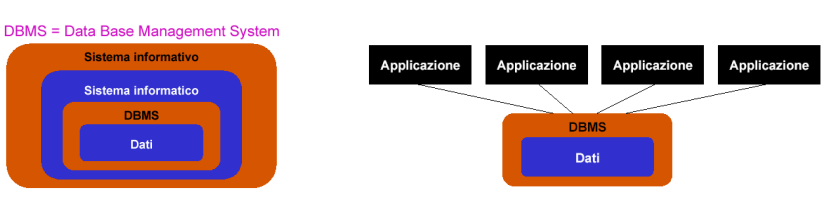
\includegraphics[width = 1\textwidth]{Images/2.PNG}
\end{center}
Le caratteristiche di una base di dati sono:
\begin{itemize}
    \item I dati sono \textbf{molti}
    \item I dati hanno un \textbf{formato definito}
    \item I dati sono \textbf{permanenti}
    \item I dati sono \textbf{raggruppati} per insiemi \textbf{omogenei} di dati
    \item Esistono \textbf{relazioni specifiche} tra gli insiemi di dati
    \item La ridondanza è \textbf{minima e controllata}: è assicurata la consistenza delle informazioni
    \item I dati sono disponibili \textbf{per utenze diverse e concorrenti}
    \item I dati sono \textbf{controllati}: protetti da malfunzionamenti hardware e software
    \item I dati della base di dati sono \textbf{indipendenti dai dati di un qualsiasi programma}
\end{itemize}
\subsection{Database Management System}
Un DBMS è un insieme di programmi che permettono di creare, usare e gestire una base di dati.
Quindi un DBMS è un sistema software general purpose che facilita il processo di \textbf{definizione, costruzione e manipolazione} del database per varie applicazioni.
Vi sono 3 fasi nella \textbf{creazione di un database}:
\begin{enumerate}
    \item \textbf{Definizione}
    \item \textbf{Creazione/Popolazione}
    \item \textbf{Manipolazione}
\end{enumerate}
Una volta creato un database, si potranno effettuare su di esso delle \textbf{interrogazioni} (queries).
L'efficacia delle queries dipende da:
\begin{itemize}
    \item Conoscenza dle contenuto del DB
    \item Esperienza con il linguaggio di interrogazione
    \item Semplicità ed efficacia dell'interfaccia di interrogazione
\end{itemize}
Un DBMS è quindi un \textbf{sistema} che gestisce collezioni di dati:
\begin{itemize}
    \item \textbf{Grandi}
    \item \textbf{Persistenti}
    \item \textbf{Condivise}
\end{itemize}
garantendo:
\begin{itemize}
    \item \textbf{Privatezza}
    \item \textbf{Affidabilità}
    \item \textbf{Efficienza}
    \item \textbf{Efficacia}
\end{itemize}
\subsection{Caratteristiche delle basi di dati}
Le basi di dato sono:
\begin{itemize}
    \item \textbf{Grandi}: dimensioni (molto) maggiori della memoria centrale dei sistemi di calcolo utilizzati. Il limite deve essere solo quello fisico dei dispositivi
    \item \textbf{Persistenti}: hanno un tempo di vita indipendente dalle singole esecuzioni dei programmi che le utilizzano
    \item \textbf{Condivise}: Ogni organizzazione (specie se grande) è divisa in settori o comunque svolge diverse attività. Ciascun settore/attività ha un (sotto)sistema informativo (non necessariamente disgiunto)
    \item I possibili problemi sono la \textbf{ridondanza}, cioè la ripetizione di informazioni, e \textbf{l'incoerenza}, cioè le varie versioni della basi di dati potrebbero non coincidere
\end{itemize}
\subsection{Archivi e basi di dati}
\begin{center}
    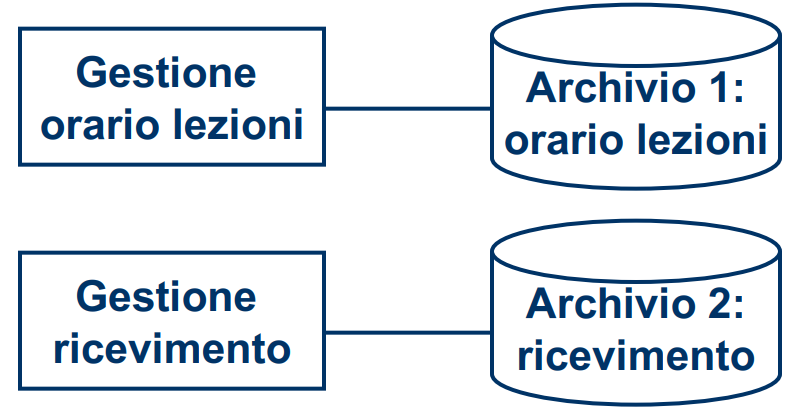
\includegraphics[width = 0.55\textwidth]{Images/3.PNG}
\end{center}
\begin{center}
    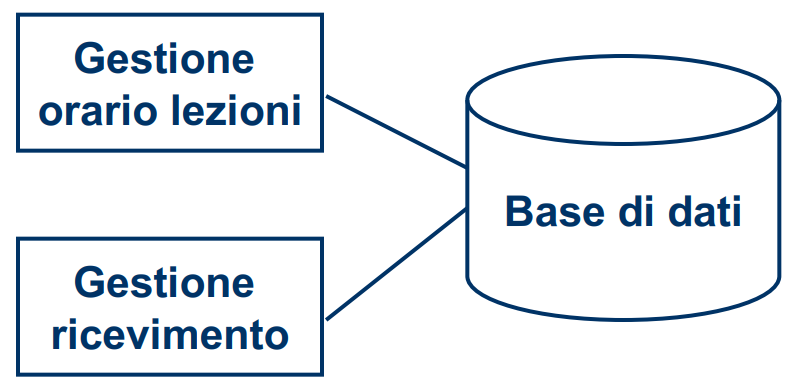
\includegraphics[width = 0.55\textwidth]{Images/4.PNG}
\end{center}
\subsection{Condivisione delle basi di dati}
Una base di dati è una risorsa \textbf{integrata e condivisa} fra applicazioni.
Diventa quindi possibile svolgere attività diverse su dati condivisi: sono necessari quindi \textbf{meccanismi di autorizzazione}.
Diventano anche possibili accessi di più utenti ai dati condivisi: sono quindi necessarie politiche e meccanismi di controllo della \textbf{concorrenza}.
\subsection{Caratteristiche dei DBMS}
I DBMS garantiscono \textbf{privatezza}; cioè si possono definire meccanismi di autorizzazione: l'utente A è, per esempio, autorizzato a leggere tutti i dati e a modificare quelli sul ricevimento; tuttavia
l'utente B è magari autorizzato a leggere i dati di X e a modificare i dati di Y. \newline
I DBMS garantiscono inoltre \textbf{l'affidabilità} dei dati, cioè la resistenza a malfunzionamenti hardware e software.
Per implementare questa caratteristica è quindi fondamentale \textbf{gestire le transazioni}.
\subsection{Transazioni}
Le \textbf{transazioni} sono l'insieme di operazioni da considerare indivisibili ("\textbf{atomiche}"), corrette anche in presenza di \textbf{concorrenza} e con effetti \textbf{definitivi}.
La sequenza di operazioni sulla base di dati viene eseguita per intero o per niente: per esempio, il trasferimento di fondi da un conto A ad un conto B avviene o tramite il prelevamento da A e il versamento su B o niente affatto.
L'effetto di transazioni concorrenti deve essere \textbf{coerente} (ad esempio "equivalente" all'esecuzione separata delle richieste concorrenti): per esempio, se due assegni emessi sullo stesso conto corrente vengono incassati \textbf{contemporaneamente},
si deve evitare di trascurarne uno.
La conclusione positiva di una transazione corrisponde ad un impegno (in inglese \textbf{commit}) a mantenere traccia del risultato in modo definitivo, anche in presenza di guasti e di esecuzione concorrente.
\subsection{Caratteristiche dei DBMS}
I DBMS devono essere \textbf{efficienti}, cioè devono cercare di utilizzare al meglio le risorse di spazio di memoria (principale e secondaria) e di tempo (di esecuzione e di risposta).
I DBMS, con tante funzioni, rischiano l'inefficienza e per questo ci sono grandi investimenti e competizione. L'efficienza è anche il risultato della qualità delle applicazioni. \newline
I DBMS devono essere \textbf{efficaci}, cioè devono cercare di rendere produttive le attività dei loro utilizzatori, offrendo funzionalità articolare, potenti e flessibili.
\subsection{Descrizioni dei dati nei DBMS}
Descrizioni e rappresentazione dei dati a livelli diversi permettono \textbf{l'indipendenza dei dati} dalla rappresentazione fisica: i programmi fanno riferimento alla struttura a livello più altro, e le rappresentazione sottostanti possono essere modificate senza necessità di modificare i programmi.
Possiamo precisare questo concetto attraverso il concetto di \textbf{modello dei dati}
\subsubsection{Modello dei dati}
Il \textbf{modello dei dati} è l'insieme di costrutti utilizzati per organizzare i dati di interesse e descriverne la dinamica.
Esso ha una componente fondamentale: i \textbf{meccanismi di strutturazione} (o \textbf{costruttori di tipo}): come nei linguaggi di programmazione
esistono meccanismi che permettono di definire nuovi tipi, così ogni modello dei dati prevede alcuni costruttori.
Ad esempio, il \textbf{modello relazionale} prevede il costruttore \textbf{relazione}, che permette di definire insiemi di record omogenei.
\subsection{Schema e istanza della base di dati}
\begin{center}
    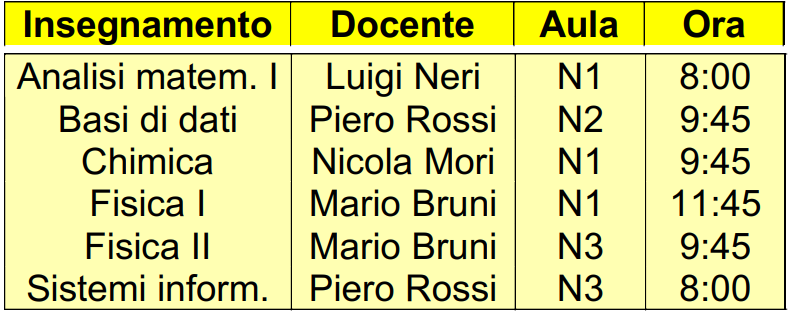
\includegraphics[width = 0.60\textwidth]{Images/5.PNG}
\end{center}
In ogni base di dati esistono:
\begin{itemize}
    \item Lo \textbf{schema}, sostanzialmente invariante nel tempo, che ne descriva la struttura e il significato (aspetto intensionale; es. le intestazioni delle tabelle). Lo schema quindi costituisce l'aspetto \textbf{intensionale}, ovvero la descrizione "astratta" delle proprietà, ed è invariante nel tempo
    \item \textbf{L'istanza}, i valori attuali, che possono cambiare anche molto rapidamente (aspetto estensionale; es. il "corpo" di ciascuna tabella). L'istanza quindi costituisce invece l'aspetto \textbf{estensionale} "concreto", che varia nel tempo al variare della situazione di ciò che stiamo descrivendo
\end{itemize}
\subsection{Modello dei dati logico}
I modelli dei dati logici sono adottati nei DBMS esistenti per l'organizzazione dei dati:
\begin{itemize}
    \item utilizzati dai programmi
    \item indipendenti dalle strutture fisiche
\end{itemize}
Esempi di essi sono il modello \textbf{relazionale}, reticolare, gerarchico, a oggetti, XML, ...
\subsubsection{Modello relazionale}
Nel modello relazionale i dati vengono strutturati in tabelle, in particolare un DBMS relazionale può essere pensato come un insieme di tabelle.
Ogni tabella mantiene informazioni di tipo omogeneo. Diverse tabelle sono collegate (in relazione) fra loro grazie alla presenza di un \textbf{campo comune}, che permette di mettere in relazione i dati delle due tabelle.
Nel modello relazionale:
\begin{itemize}
    \item \textbf{Lo schema} è la descrizione della struttura delle tabelle (stabile nel tempo)
    \item \textbf{L'istanza} sono i valori dei campi della tabella
\end{itemize}
\begin{center}
    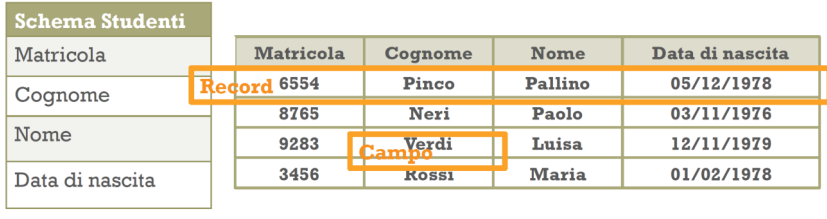
\includegraphics[width = 0.85\textwidth]{Images/6.PNG}
\end{center}
\subsection{Modello dei dati concettuale}
I modelli dei dati concettuali permettono di rappresentare i dati in modo indipendente da ogni sistema.
\begin{itemize}
    \item cercando di descrivere i concetti del mondo reale
    \item sono utilizzati nelle fasi preliminare di progettazione (quali informazioni sono utili? Come sono collegate?)
\end{itemize}
Il più diffuso è il modello \textbf{Entity-Relationship}
\newpage
\subsection{Architettura di un DBMS}
Possiamo strutturare l'architettura di un DBMS in maniera \textbf{semplificata} nel seguente modo:
\begin{center}
    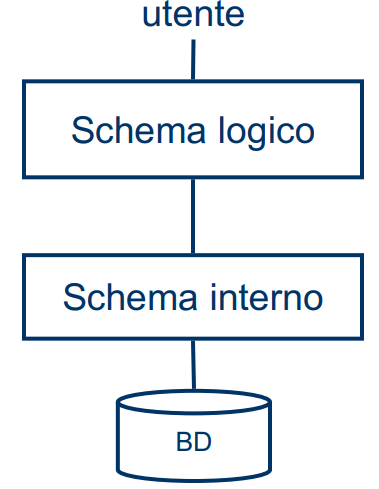
\includegraphics[width = 0.35\textwidth]{Images/7.PNG}
\end{center}
Nella quale:
\begin{itemize}
    \item \textbf{Schema logico}: descrizione della base di dati nel modello logico (ad esempio, la struttura della tabella)
    \item \textbf{Schema interno (o fisico)}: rappresentazione dello schema logico per mezzo di strutture di memorizzazione (file ad esempio, ma anche record con puntatori, ordinati in un certo modo)
\end{itemize}
Una delle architetture standard di riferimento per i DBMS è \textbf{L'architettura \newline ANSI/SPARC a tre livelli}:
\begin{center}
    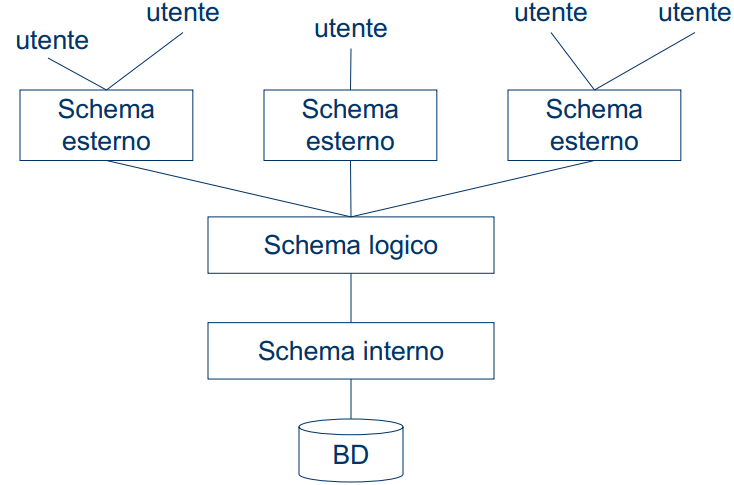
\includegraphics[width = 0.65\textwidth]{Images/8.PNG}
\end{center}
Nella quale:
\begin{itemize}
    \item \textbf{Schema logico}; descrizione dell'intera base di dati nel modello logico "principale" del DBMS
    \item \textbf{Schema fisico}: rappresentazione dello schema logico per mezzo di strutture fisiche di memorizzazione
    \item \textbf{Schema esterno}: descrizione di parte della base di dati in un modello logico ("viste" parziali, derivate, anche in modelli diversi)
\end{itemize}
\begin{center}
    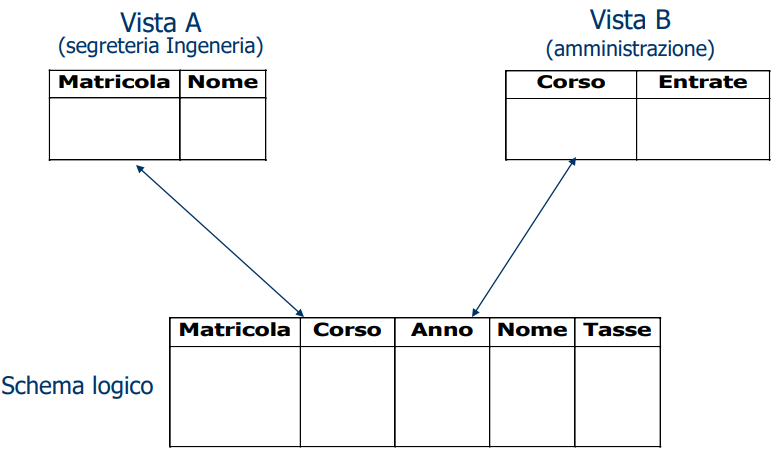
\includegraphics[width = 0.75\textwidth]{Images/9.PNG}
\end{center}
\subsection{Indipendenza dei dati}
Il livello logico è indipendente da quello fisico: una tabella è utilizzata nello stesso modo qualunque sia la sua realizzazione fisica (che può anche cambiare nel tempo).
In questo corso vedremo solo il livello logico e non quello fisico.
La conseguenza della articolazioni in livelli è che l'accesso avviene solo tramite il \textbf{livello esterno} (che può coincidere con il livello logico).
Vi sono due forme di indipendenza:
\begin{itemize}
    \item \textbf{Indipendenza fisica}
    \item \textbf{Indipendenza logica}
\end{itemize}
\subsubsection{Indipendenza fisica}
Il livello logico e quello esterno sono indipendenti da quello fisico. Una relazione è utilizzata nello stesso modo qualunque sia la sua realizzazione fisica.
La realizzazione fisica può cambiare senza che debbano essere modificati i programmi che usano la base di dati.
\subsubsection{Indipendenza logica}
Il livello esterno è indipendente da quello logico. Aggiunte o modifiche alle viste non richiedono modifiche al livello logico.
Le modifiche allo schema logico che lasciano inalterato lo schema esterno sono quindi \textbf{trasparenti}.
\subsection{Linguaggi per basi di dati}
Vi sono due tipi di linguaggi per le basi di dati:
\begin{itemize}
    \item \textbf{Data Definition Languages}(DDL): Servono a definire degli schemi logici, fisici e delle autorizzazioni di accesso
    \item \textbf{Data Manipulation Languages}(DML): Servono per effettuare l'interrogazione e l'aggiornamento delle basi di dati 
\end{itemize}
Alcuni linguaggi come SQL (Structured Query Language) hanno funzioni di entrambe le categorie.
\subsection{Personaggi e interpreti}
Si possono identificare diverse figure durante l'intero ciclo di vita di una base di dati:
\begin{itemize}
    \item \textbf{Progettisti} e realizzatori di \textbf{DBMS}
    \item \textbf{Progettisti della base di dati} e amministratori della base di dati (\textbf{DBA})
    \item \textbf{Progettisti} e programatori di \textbf{Applicazioni}
    \item \textbf{Utenti}
    \begin{itemize}
        \item Utenti \textbf{finali}(terminalisti): eseguono applicazioni predefinite(\textbf{transazioni})
        \item Utenti \textbf{casuali}: eseguono operazioni non previste a priori, usando linguaggi interattivi
    \end{itemize}
\end{itemize}
\subsubsection{Database administrator (DBA)}
Un \textbf{database administrator}(DBA) è una persona o gruppo di persone responsabile del controllo centralizzato e della gestione del sistema, delle prestazioni, dell'affidabilità e delle autorizzazioni.
Le funzioni del DBA includono quelle di progettazione, anche se in progetti complessi ci possono essere distinzioni.
\subsubsection{Utenti del DBMS}
\begin{center}
    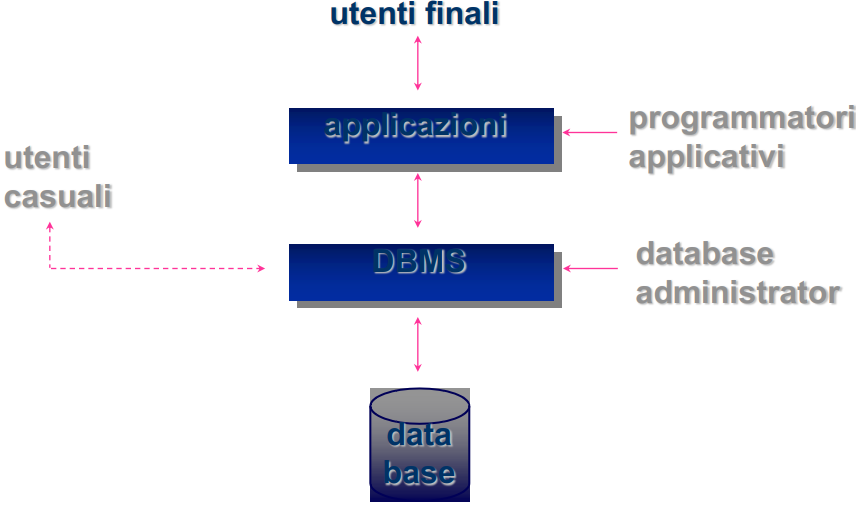
\includegraphics[width = 0.75\textwidth]{Images/10.PNG}
\end{center}
\subsection{Vantaggi e svantaggi dei DBMS}
Vediamo quali sono i \textbf{vantaggi} di avere un DBMS:
\begin{itemize}
    \item Permettono di considerare i dati come risorsa comune di un'organizzazione, a disposizione di molteplici applicazioni e utenti
    \item Offrono un modello della parte di mondo di interesse che è unificato e preciso, utilizzabile in applicazioni attuali e future
    \item Offrono un controllo centralizzato dei dati, riducendo ridondanze e inconsistenze
    \item Permettono l'indipendenza dei dati: favoriscono lo sviluppo di applicazioni flessibili e facilmente modificabili
\end{itemize}
Vediamo quali sono invece gli \textbf{svantaggi} di avere un DBMS:
\begin{itemize}
    \item Un DBMS è costoso, complesso e ha specifici requisiti in termini di software e hardware
    \item Diventa difficile separare, tra tutti i servizi offerti da un DBMS, quelli effettivamente usati da quelli inutili
    \item Sono inadatti alla gestione di applicazioni con pochi utenti (NB: Dipende dai costi operativi)
\end{itemize}
\subsection{Caratteristiche dell'approccio con basi di dati}
L'approccio alla \textbf{rappresentazione dei dati tramite basi di dati} ha le seguenti caratteristiche:
\begin{itemize}
    \item \textbf{Astrazione dei dati}: si usa un \textbf{modello dati} per nascondere dettagli e presentare all'utente una \textit{vista concettuale} del database
    \item \textbf{Supporto di viste multiple dei dati}: Ogni utente può usare una vista (view) differente del database, contente solo i dati di interesse per quell'utente
\end{itemize}
\section{Progettazione di unaa base di dati}
La \textbf{progettazione di basi di dati} è una delle attività del processo di sviluppo dei sistemi informativi e va quindi inquadrata in un contesto più generale: \textbf{il ciclo di vita dei sistemi informativi}.
\subsection{Ciclo di vita dei sistemi informativi}
Il ciclo di vita dei sistemi informativi è \textbf{l'insieme e sequenzializzazione delle attività svolte da analisti, progettisti, utenti nello sviluppo e nell'uso dei sistemi informativi}.
È un attività iterativa, quindi è un "ciclo".
\newpage
\noindent
Le fasi del ciclo di vita sono:
\begin{center}
    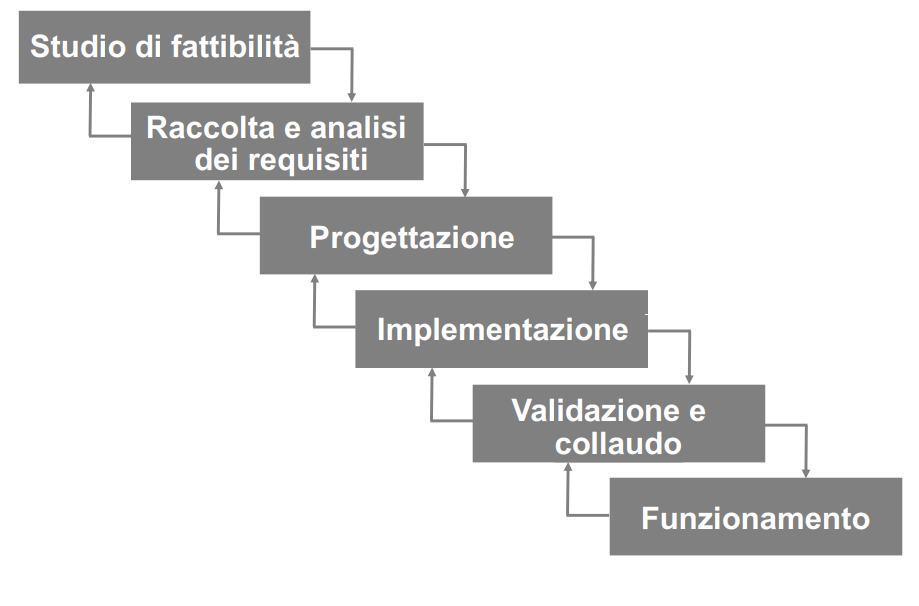
\includegraphics[width = 0.85\textwidth]{Images/11.PNG}
\end{center}
Diamone una definizione:
\begin{itemize}
    \item \textbf{Studio di fattibilità}: definizione dei costi e delle priorità
    \item \textbf{Raccolta e analisi dei requisiti}: studio delle proprietà del sistema
    \item \textbf{Progettazione}: di dati e funzioni
    \item \textbf{Validazione e collaudo}: sperimentazione
    \item \textbf{Funzionamento}: il sistema diventa operativo
\end{itemize}
Possiamo anche rappresentare questo ciclo di vita come una spirale:
\begin{center}
    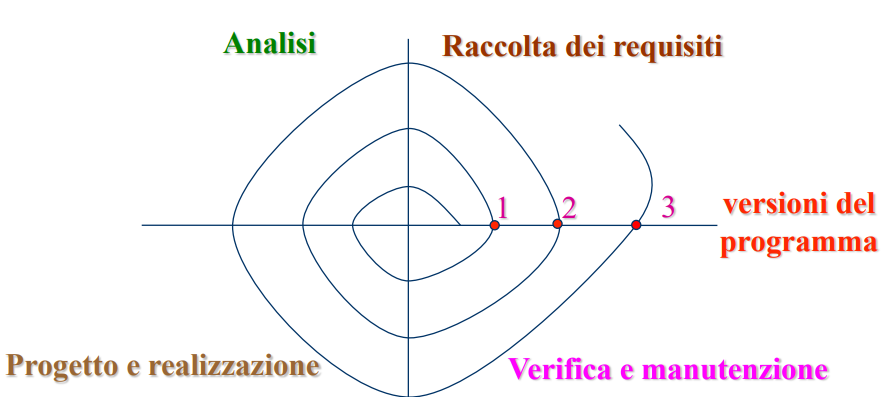
\includegraphics[width = 0.85\textwidth]{Images/12.PNG}
\end{center}
\subsubsection{Progettazione}
La progettazione dei dati individua l'organizzazione e la struttura della base di dati.
La progettazione delle applicazioni schematizza le operazioni sui dati e progetta il software applicativo.
I dati hanno \textbf{un ruolo centrale} e grazie alla progettazione:
\begin{itemize}
    \item i dati sono \textbf{più stabili}
    \item Si progetta prima la base di dati e poi le applicazioni
\end{itemize}
\subsubsection{Metodologia di progettazione}
Per garantire prodotti di buona qualità è opportuno seguire \textbf{una metodologia di progetto}; cioè un'articolazione in fasi/passi di guida ad una attività di progettazione.
Serve una metodologia di progettazione (insieme di strumenti) che:
\begin{itemize}
    \item permetta di \textbf{suddividere} la progettazione in fasi successive indipendenti
    \item fornisca \textbf{strategie} da seguire e criteri di scelta in caso di alternative
    \item fornisca \textbf{modelli di riferimento (linguaggi)} per descrivere la realtà che stiamo progettando
\end{itemize}
e che garantisca:
\begin{itemize}
    \item \textbf{Generalità} rispetto ai problemi da affrontare
    \item \textbf{Qualità} in termini di correttezza, completezza ed efficienza
    \item \textbf{Facilità d'uso}
\end{itemize}
Una metodologia di progettazione di basi di dati si basa su un principio semplice ma efficace:
\textbf{la separazione netta tra decisioni relative a}:
\begin{itemize}
    \item \textbf{Come rappresentare}
    \item \textbf{Come farlo}
\end{itemize}
\begin{center}
    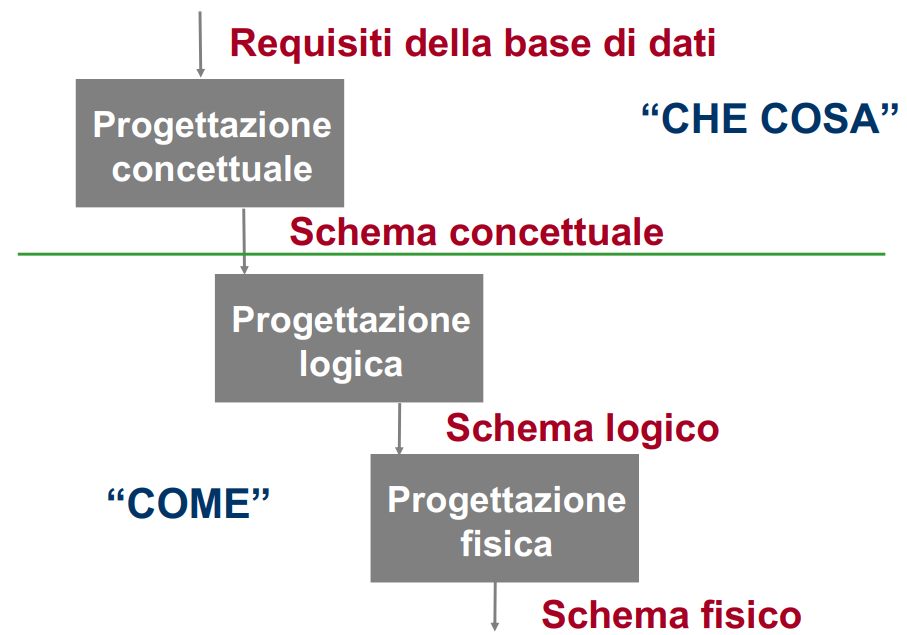
\includegraphics[width = 0.80\textwidth]{Images/13.PNG}
\end{center}
La metodologia introdotta prevede 3 fasi:
\begin{itemize}
    \item Progettazione \textbf{concettuale}
    \item Progettazione \textbf{logica}
    \item Progettazione \textbf{fisica}
\end{itemize}
Ognuna delle fasi si basa su un \textbf{modello}, che permette di generare una rappresentazione formale (schema) della base di dati ad un dato livello di astrazione (concettuale, logico e fisico):
\begin{itemize}
    \item Schema concettuale
    \item Schema logico
    \item Schema fisico
\end{itemize}
\subsubsection{Fase di progettazione concettuale}
La fase diu progettazione concettuale traduce i requisiti del sistema informatico in una descrizione \textbf{formalizzata e integrata} delle esigenze aziendali, espressa in modo \textbf{indipendente} dalle scelte implementative (DBMS, SW e HW).
Essa è:
\begin{itemize}
    \item \textbf{Formale}: la descrizione deve essere espressa con un linguaggio non ambiguo e capace di descrivere in modo soddisfacente il sistema analizzato
    \item \textbf{Integrata}: la descrizione deve essere in grado di descrivere nella globalità l'ambiente analizzato
    \item \textbf{Indipendente dall'ambiente tecnologico}: la descrizione deve concentrarsi sui dati e sulle loro relazioni e non sulle scelte implementative
\end{itemize}
\subsubsection{Fase di progettazione logica}
La progettazione logica consiste nella traduzione dello schema concettuale nel modello dei dati del DBMS.
Il risultato è uno schema logico, espresso nel DDL del DBMS.
In questa fase si considerano anche aspetti legati ai vincoli e all'efficienza.
La progettazione logica si articola in due sotto-fasi:
\begin{itemize}
    \item \textbf{Ristrutturazione dello schema concettuale}
    \item \textbf{Traduzione verso il modello logico}
\end{itemize}
\subsubsection{Progettazione fisica}
La progettazione fisica completa lo schema logico ottenuto con le specifiche proprie dell'hw/sw scelto.
Il risultato è lo \textbf{schema fisico} che descrive le strutture di memorizzazione ed accesso ai dati.
\subsubsection{Vantaggi della progettazione concettuale}
La progettazione concettuale permette una descrizione dei dati indipendete degli aspetti tecnologici con un livello di astrazione intermedio fra utente e sistema.
\textbf{Prevale l'aspetto intensionale}.
Inoltre, essa utilizza una rappresentazione prevalentemente \textbf{grafica}, che migliora la comunicazione tra i progettisti, gli utenti e tutte le persone coinvolte nella realizzazione dell'applicazione.
È inoltre utile per la \textbf{documentazione}.
\begin{center}
    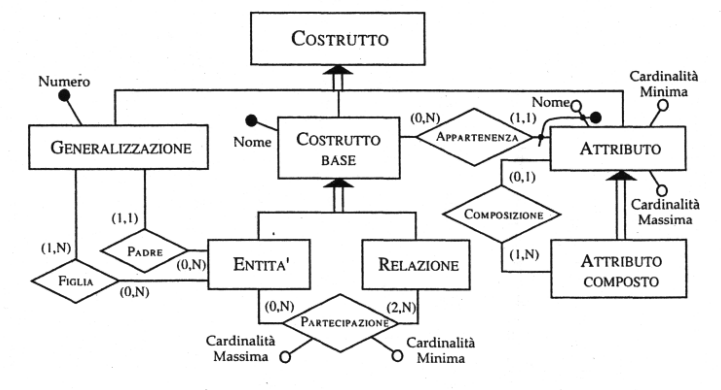
\includegraphics[width = 0.80\textwidth]{Images/14.PNG}
\end{center}
\section{Modello Entità-Relazione (E-R)}
Il modello entità-relazione (E-R) è un linguaggio grafico semi-formale per la rappresentazione di schemi concettuali.
Il modello E-R si è ormai affermato come uno standard nelle metodologie di progetto e nei sistemi SW di ausilio alla progettazione.
Ne esistono molte versione più o meno diverse l'una dall'altra.
\subsection{Introduzione ai costrutti}
\begin{center}
    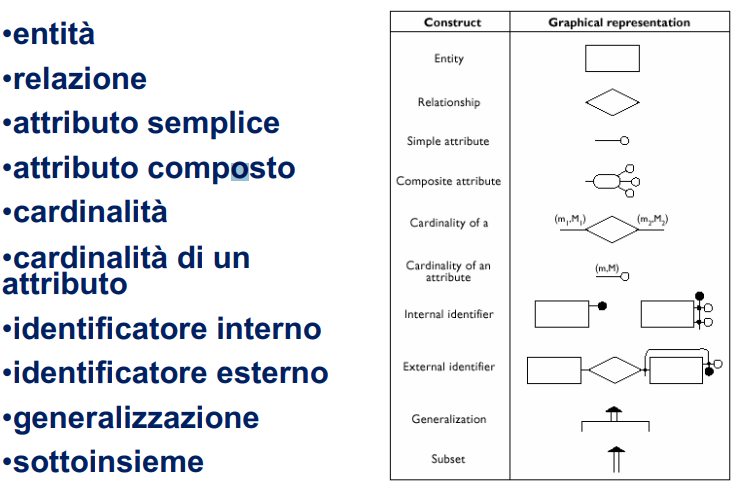
\includegraphics[width = 0.81\textwidth]{Images/15.PNG}
\end{center}
\subsection{Entità}
Un'entità è una classe di oggetti (fatti, persone, cose) della applicazione di interesse con proprietà comuni e con esistenza \textbf{autonoma} e della quale si vogliono registrare fatti specifici.
Per esempio, un'entità potrebbe essere un impiegato, un dipartimento, una città, un conto corrente, un'università, uno studente, ...
Graficamente le entità si rappresentano nel seguente modo:
\begin{center}
    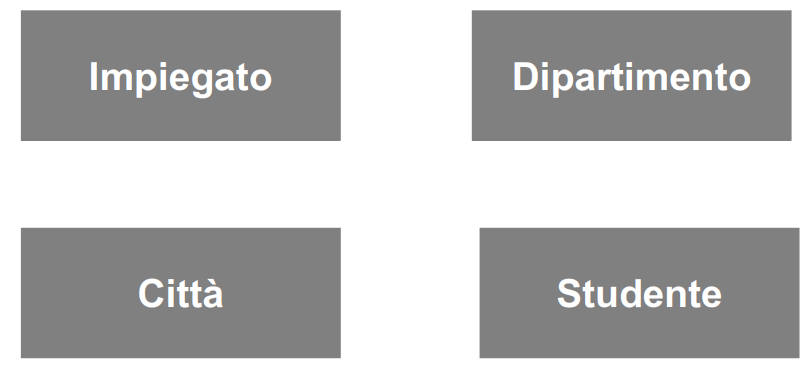
\includegraphics[width = 0.70\textwidth]{Images/16.PNG}
\end{center}
Ogni entità ha un nome che la identifica univocamente nello schema, il quale deve essere:
\begin{itemize}
    \item \textbf{Espressivo}
    \item \textbf{Al singolare}
\end{itemize}
A livello \textbf{estensionale} un'entità è costituita da un insieme di oggetti, che sono chiamati le sue \textbf{istanze}.
Ciò significa che, se in uno schema $S$ è definita una entità $E$, in ogni istanza $I$ dello schema $S$, alla entità $E$ è associato un insieme di oggetti
$$istanze(I,E) = \{e_1, e_2, e_3, \dots\}$$
che viene detto anche \textit{l'estensione} di $E$ nella istanza $I$ dello schema $S$.
Una istanza di entità non è un valore che identifica un oggetto, ma è \textbf{l'oggetto stesso}.
Quindi ogni istanza di entità è \textbf{oggetto della classe che l'entità rappresenta}.
Nello schema concettuale rappresentiamo le \textbf{entità}, non le singole istanze ("astrazione").
Quindi:
\begin{itemize}
    \item \textbf{Conoscenza astratta}: entità
    \item \textbf{Conoscenza concreta}: istanza di entità
\end{itemize}
\subsection{Attributi}
Un attributo di entità è una proprietà locale di un'entità, di interesse ai fini dell'applicazione.
Un attributo associa ad ogni istanza di entità un valore appartenente ad un insieme detto \textbf{dominio dell'attributo} (tipicamente interi, caratteri, stringhe, ecc\dots).
Si definisce quindi un attributo per l'entità $E$ quando si vuole rappresentare una proprietà \textbf{locale} delle istanze dell'entità $E$.
Una proprietà di un oggetto si dice locale quando in ogni istanza dello schema il valore di tale proprietà dipende \textbf{solamente} dall'oggetto stesso e \textbf{non ha alcun rapporto} con altri elementi dell'istanza dello schema.
Nel modello E-R, gli attributi si rappresentano nella seguente maniera:
\begin{center}
    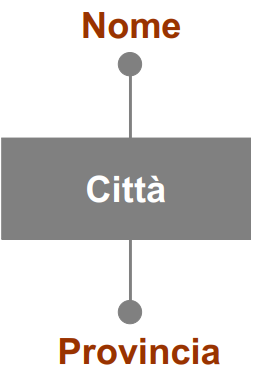
\includegraphics[width = 0.25\textwidth]{Images/17.PNG}
\end{center}
Ogni attributo di entità ha un nome che lo identifica in modo univoco nell'ambito dell'entità, ed è rappresentato da un cerchio collegato alla entità a cui appartiene.
Ogni attributo è definito su un dominio di valori. Un attributo associa ad ogni istanza di entità o associazione un valore nel corrispondente dominio.
I domini solitamente non vengono specificati nell'E-R ma nella documentazione associata. Se li si vuole indicare, la notazione è la seguente:
\begin{center}
    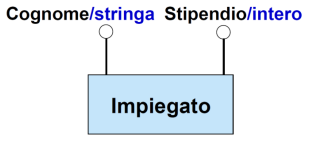
\includegraphics[width = 0.50\textwidth]{Images/18.PNG}
\end{center}
Quindi, ogni attributo può essere pensato come una vera e propria \textbf{funzione} che associa una determinata istanza di un'entità ad un particolare valore per quell'attributo;
di conseguenza \textbf{valgono tutte le definizioni e tutte le proprietà delle funzioni}
\begin{center}
    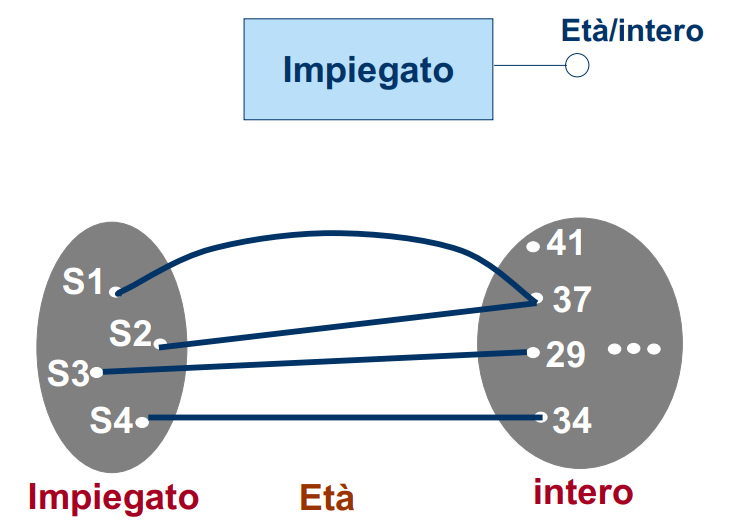
\includegraphics[width = 0.65\textwidth]{Images/19.PNG}
\end{center}
Inoltre, un'attributo è una \textbf{funzione totale}, quindi ogni istanza di un'entità deve avere un valore associato per ogni suo attributo.
\subsection{Attributi composti}
Gli attributi composti si ottengono raggruppando attributi di una medesima entità o relazione che presentano affinità nel loro significato o uso:
\begin{center}
    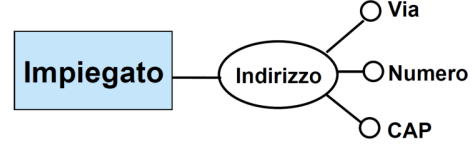
\includegraphics[width = 0.40\textwidth]{Images/20.PNG}
\end{center}
\subsection{Relazioni}
Una relazione è un fatto che descrive un'azione o una situazione che \textbf{stabilisce legami logici} tra istanze di entità (associa, mette in relazione) nella
\textbf{realtà che stiamo considerando}.
\textbf{I legami possono essere fra più di due entità}. Il numero di entità coinvolte in una relazione determina il suo \textbf{grado}.
Nel modello E-R una relazione si indica nel seguente modo:
\begin{center}
    
\includegraphics[width = 0.65\textwidth]{Images/21.PNG}
\end{center}
Ogni relazione ha un nome che la identifica univocamente nello schema ed esso deve essere:
\begin{itemize}
    \item \textbf{Espressivo}
    \item \textbf{Singolare} e usare \textbf{sostantivi invece che verbi}
\end{itemize}
A livello \textbf{estensionale} una relazione $R$ tra le entità $E$ ed $F$ è costituita da un insieme di coppie $(x,y)$, tali che $x$ è una istanza di $E$ ed $y$ è un istanza di $F$.
Ogni coppia è detta \textbf{istanza} della relazione $R$.
cIò significa che, se in uno schema $S$ è definita una relazione $R$ sulle entità $E$ ed $F$, in ogni istanza $I$ dello schema $S$, alla relazione $R$ è associato un insieme di coppie
(denotato da istanze $(I, R)$)
$$\{(x_1, y_1) (x_2, y_2), (x_3, y_3), \dots\}$$
che viene detto anche \textit{l'estensione} di $R$ nella istanza $I$ dello schema $S$.
In altre parole, una relazione nel modello E-R è, dal punto di vista della semantica, una relazione matematica.
In ogni istanza $I$ dello schema $S$ si ha:
$$istanze(I, R) \subseteq istanze(I,E) \times istanze(I,F)$$
In particolare si dice \textbf{istanza di un'associazione} la combinazione (aggregazione) di istanze di entità che prendono parte alla associazione.
Dalla semantica delle relazioni segue immediatamente che \textbf{non} possono esistere due istanze della stessa relazione che coinvolgono le stesse istanze di entità.
\newpage
\noindent
Tuttavia \textbf{due entità possono essere coinvolte in più associazioni}:
\begin{center}
    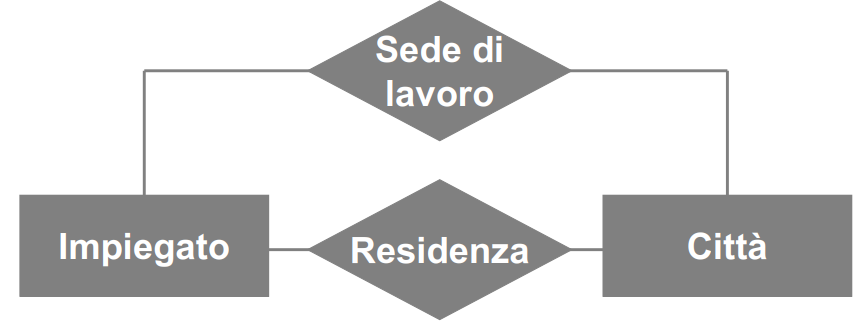
\includegraphics[width = 0.65\textwidth]{Images/22.PNG}
\end{center}
Inoltre le relazioni possono coinvolgere più di due entità:
\begin{center}
    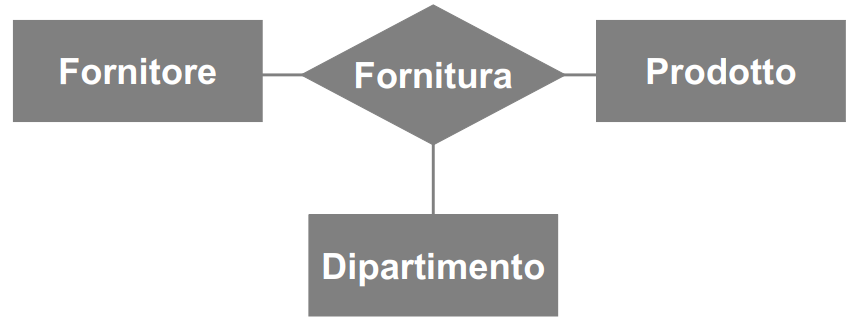
\includegraphics[width = 0.65\textwidth]{Images/23.PNG}
\end{center}
\begin{center}
    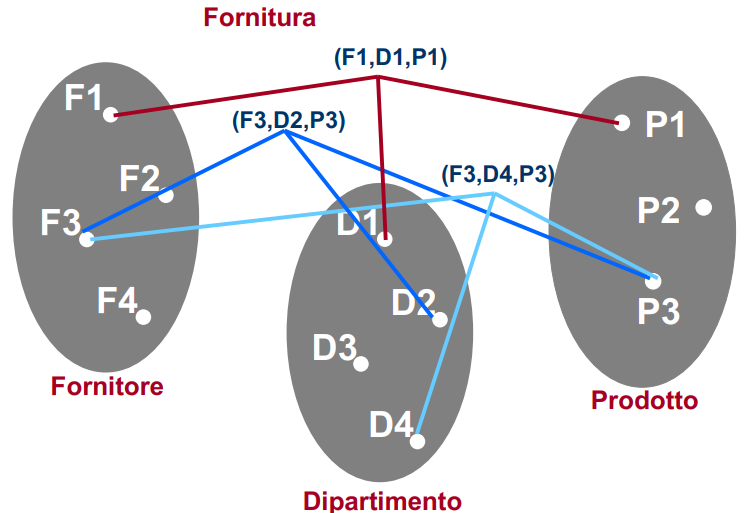
\includegraphics[width = 0.65\textwidth]{Images/24.PNG}
\end{center}
Se si parla quindi di una relazione \textbf{n-aria}, a livello \textbf{estensionale} (ovvero in ogni istanza $I$ dello schema $S$) una relazione $R$ tra le entità
$E_1, E_2, \dots, E_n$ è costituita dun insieme di n-uple (o tuple) $(x_1, x_2, \dots, x_n)$, tali che $x_1$ è un istanza di $E_1$ in $I$, $x_2$ è un istanza di $E_2$ in $I$, \dots
$x_N$ è un istanza di $E_n$ in $I$.
Ogni n-upla è detta \textbf{istanza} della relazione $R$ nella istanza $I$ dello schema $S$.
Quindi, in ogni istanza $I$ dello schema si ha:
$$istanze(I,R) \subseteq istanze(I, E_1) \times \dots \times istanze(I, E_n)$$
\subsection{Attributi di relazione}
Un attributo di relazione è una proprietà locale di una relazione, di interesse ai fini dell'applicazione.
Un attributo della relazione $R$ tra le entità $E_1, E_2, \dots, E_n$ modella una proprietà \textbf{non} propria delle entità
ma del \textbf{legame} tra le varie entità rappresentato da $R$.
Un attributo associa ad ogni istanza di relazione un valore appartenente ad un insieme detto \textbf{dominio} dell'attributo.
Ogni attributo di relazione ha un nome che lo identifica in modo univoco nell'ambito della relazione, ed è rappresentato da un cerchio collegato alla relazione a cui appartiene.
\begin{center}
    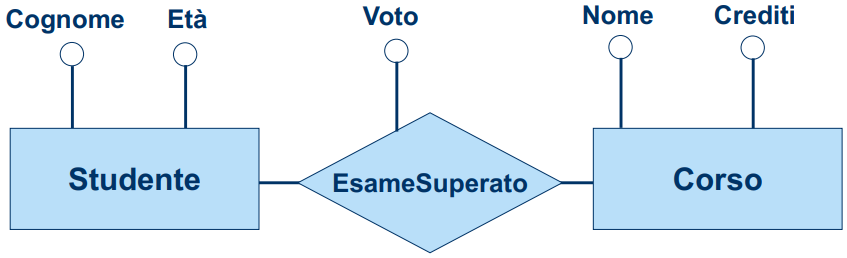
\includegraphics[width = 0.70\textwidth]{Images/25.PNG}
\end{center}
\begin{center}
    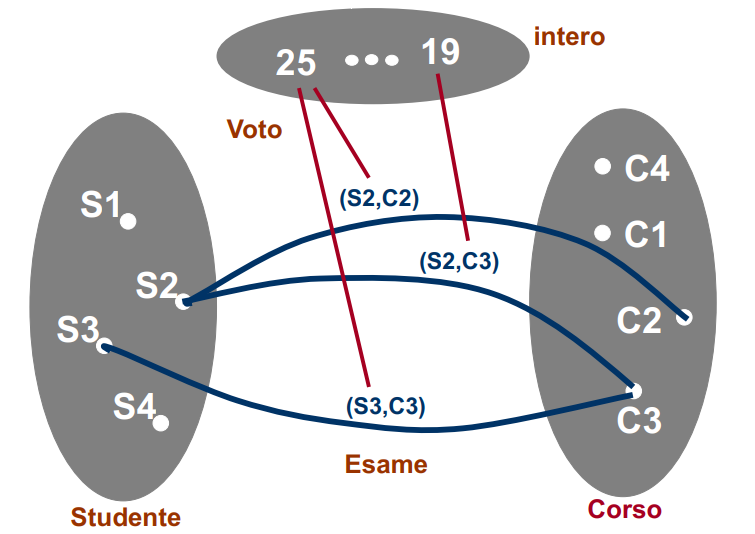
\includegraphics[width = 0.70\textwidth]{Images/26.PNG}
\end{center}
Ovviamente gli attributi possono essere presenti su associazioni n-arie:
\begin{center}
    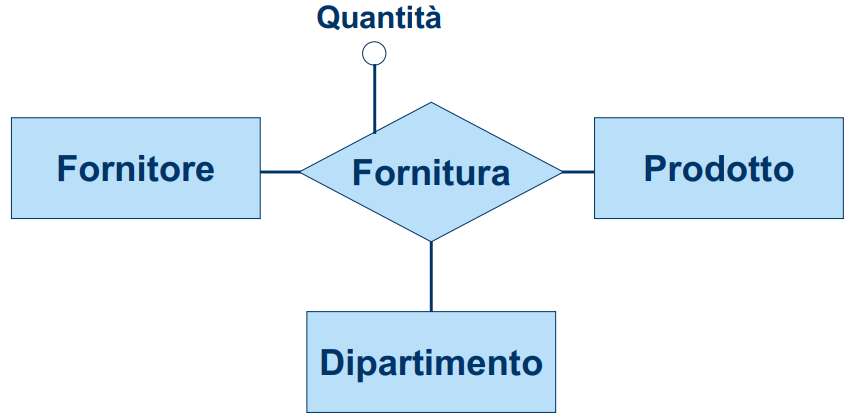
\includegraphics[width = 0.75\textwidth]{Images/27.PNG}
\end{center}
\begin{center}
    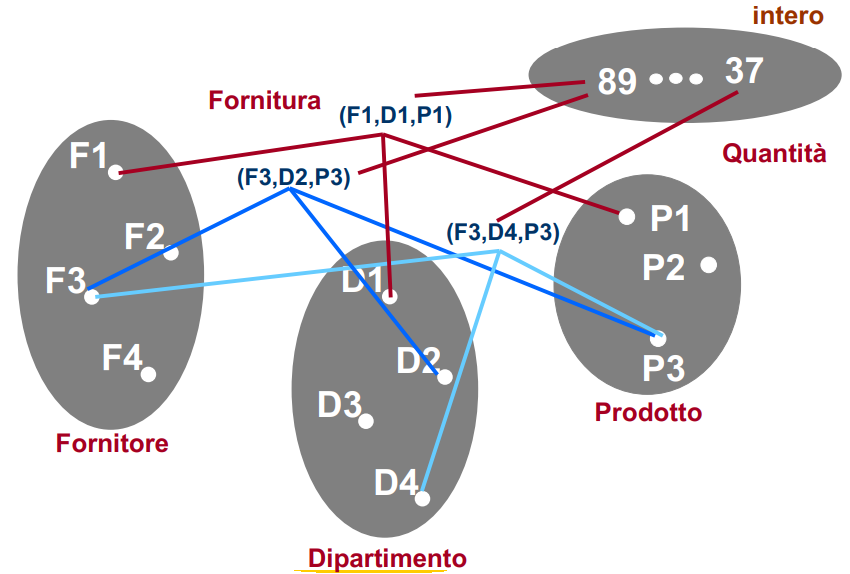
\includegraphics[width = 0.75\textwidth]{Images/28.PNG}
\end{center}
\subsection{Analisi dei casi dubbi}
I nomi di entità e associazioni alle volte traggono in inganno: è bene quindi, nel caso si presentino situazioni poco chiare, bisogna provare a ragionare anche in termini di istanze:
cosa "contiene" effettivamente questa entità/associazione?
\subsection{Relazioni ricorsive}
Una associazione può coinvolgere "due o più volte" la stessa entità:
\begin{center}
    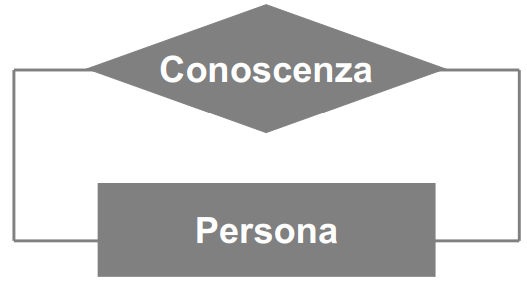
\includegraphics[width = 0.40\textwidth]{Images/29.PNG}
\end{center}
Vi è però il problema di \textbf{identificare i ruoli in questa associazione}.
Per farlo, essi si scrivono di fianco ai "collegamenti" che collegano la relazione con l'entità:
\begin{center}
    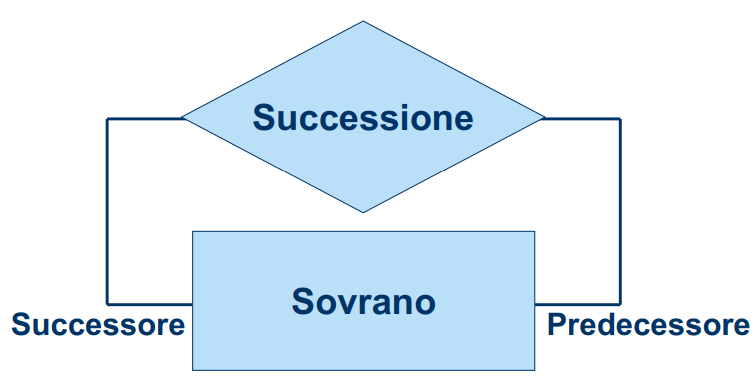
\includegraphics[width = 0.60\textwidth]{Images/30.PNG}
\end{center}
\newpage
\noindent
Un'associazione ricorsiva può essere o meno:
\begin{itemize}
    \item \textbf{Simmetrica}: $(a,b) \in A \Rightarrow (b,a) \in A$
    \item \textbf{Riflessiva}: $(a,a) \in A$
    \item \textbf{Transitiva}: $(a,b) \in A, (b,c) \in A \Rightarrow (a,c) \in A$
\end{itemize}
Una associazione ricorsiva può essere anche n-aria:
\begin{center}
    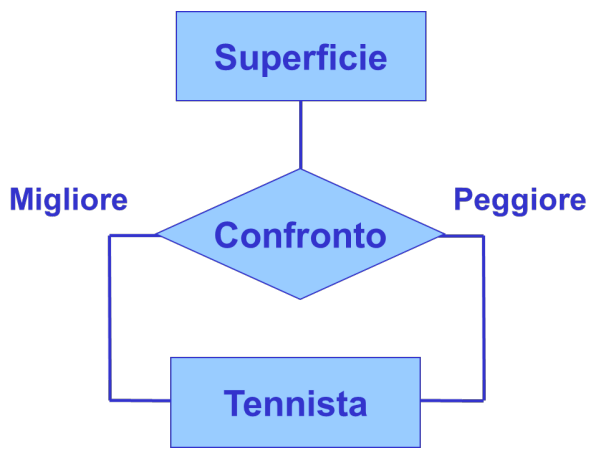
\includegraphics[width = 0.30\textwidth]{Images/31.PNG}
\end{center}
\subsection{Scelta tra entità, relazione e attributo}
Un concetto verrà modellato come:
\begin{itemize}
    \item \textbf{Entità}:
    \begin{itemize}
        \item Se le sue istanze sono concettualmente significative indipendentemente da altre istanze
        \item Se ha o potrà avere delle proprietà indipendenti dagli altri concetti
        \item Se il concetto è importante nell'applicazione
    \end{itemize}
    \item \textbf{Attributo} di un'entità o di una relazione:
    \begin{itemize}
        \item Se le sue istanze non sono concettualmente significative
        \item Se non ha senso considerare una sua istanza indipendentemente da altre istanze
        \item Se serve solo a rappresentare una proprietà locale di un altro concetto
    \end{itemize}
    \item \textbf{Relazione}:
    \begin{itemize}
        \item Se le sue istanze non sono concettualmente significative indipendentemente da altre istanze, cioè le sue istanze rappresentano n-uple di altre istanze
        \item Se non ha senso pensare alla partecipazione delle sue istanze ad altre relazioni
    \end{itemize}
\end{itemize}
Le scelte che si prendono possono cambiare durante l'analisi.
\subsection{Cardinalità}
La cardinalità è una coppia di valori che si associa a ogni entità che partecipa a una relazione.
Specificano il numero minimo e massimo di occorrenze della relazione cui ciascuna occorrenza di una entità può partecipare.
Per semplicità usiamo solo tre simboli:
\begin{itemize}
    \item 0 e 1 per la cardinalità \textbf{minima}
    \begin{itemize}
        \item 0 = "partecipazione \textbf{opzionale}"
        \item 1 = "partecipazione \textbf{obbligatoria}"
    \end{itemize}
    \item 1 e "N" per la \textbf{massima}; con N che non pone alcun limite
\end{itemize}
Nel modello E-R le cardinalità si rappresentano nel seguente modo:
\begin{center}
    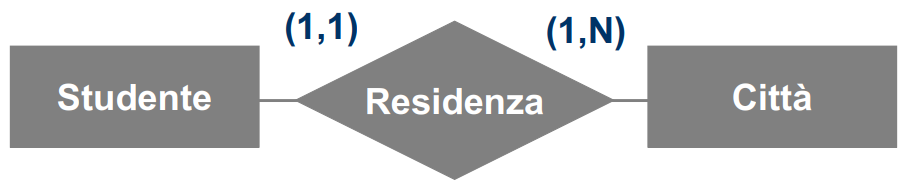
\includegraphics[width = 0.65\textwidth]{Images/32.PNG}
\end{center}
Con riferimento alle cardinalità \textbf{massime}, abbiamo relazioni:
\begin{itemize}
    \item \textbf{Uno a uno}: se le cardinalità massime di entrambe le entità sono uno
    \item \textbf{Uno a molti}: se la cardinalità massima associata ad un'entità è 1 e la cardinalità massima associata all'altra entità è N 
    \item \textbf{Molti a molti}: se le cardinalità massime per entrambe le entità è N
\end{itemize}
\subsubsection{Vincoli di cardinalità}
Un \textbf{vincolo di cardinalità} tra un'entità $E$ e una relazione $R$ esprime un limite minimo (\textbf{cardinalità minima})
ed un limite massimo (\textbf{cardinalità massima}) di istanze della relazione $R$ a cui può partecipare ogni istanza dell'entità $E$.
Serve a caratterizzare meglio il significato di una relazione.
\subsubsection{Cardinalità di attributi}
È possibile associare delle cardinalità anche agli attributi, con due scopi:
\begin{itemize}
    \item Indicare \textbf{opzionalità}
    \item Indicare \textbf{attributi multivalore}
\end{itemize}
\begin{center}
    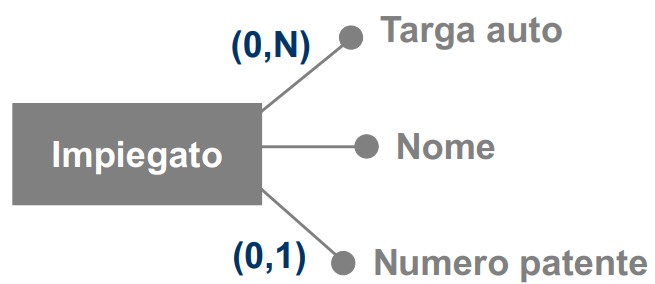
\includegraphics[width = 0.65\textwidth]{Images/33.PNG}
\end{center}
\subsection{Identificatori di un'entità}
L'identificatore è uno "strumento" per l'identificazione univoca delle occorrenze di un'entità.
Esso è costituito da
\begin{itemize}
    \item \textbf{Attributi dell'entità}; in questo caso è detto \textbf{identificatore interno}
    \item \textbf{Attributi dell'entità più entità esterne attraverso relazioni}; in questo caso è detto \textbf{identificatore esterno}
\end{itemize}
Per gli \textbf{identificatori interni} si segue la seguente notazione:
\begin{itemize}
    \item Se l'identificatore è formato da un solo attributo, si annerisce il corrispondente pallino
    \item Se l'identificatore è formato da più attributi, si uniscono gli attributi con una linea che termina con pallino annerito
\end{itemize}
\begin{center}
    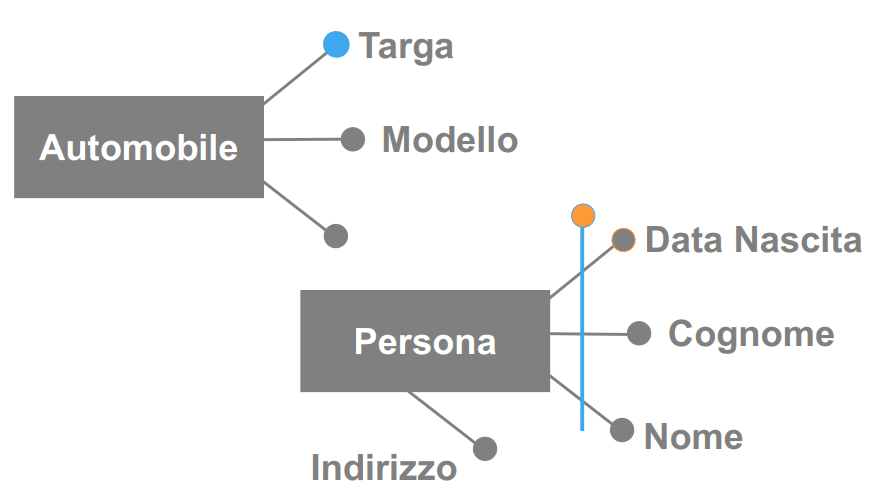
\includegraphics[width = 0.65\textwidth]{Images/34.PNG}
\end{center}
Per gli \textbf{identificatori esterni} si segue la seguente notazione:
\begin{itemize}
    \item Se l'identificatore è formato da attributi e relazioni (o meglio, ruoli), si indica unendo gli attributi ed i ruoli con una linea che termina con pallino annerito.
    \item Una identificazione esterna è possibile solo \textbf{attraverso una relazione a cui l'entità da identificare partecipa con cardinalità (1,1)}
\end{itemize}
\begin{center}
    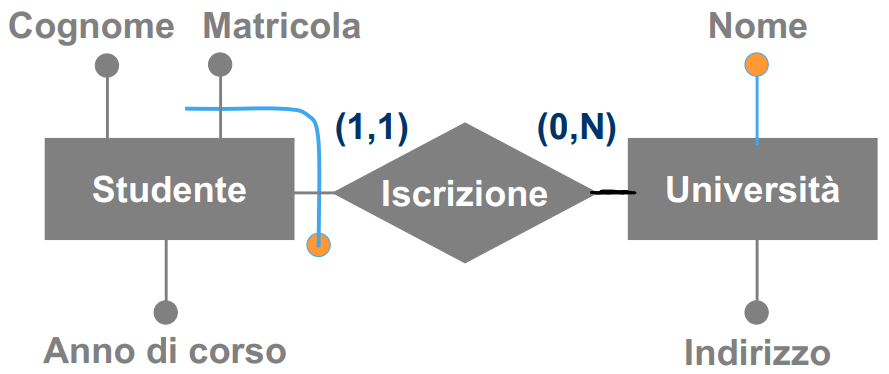
\includegraphics[width = 0.65\textwidth]{Images/35.PNG}
\end{center}
Ogni entità deve possedere almeno un identificatore, ma può averne in generale più di uno.
\subsection{Relazione IS-A tra entità}
Fino ad ora non abbiamo detto nulla sul fatto se due entità possano o no avere istanze in comune.
È facile verificare che, in molti contesti, può accadere che tra due classi rappresentate da due entità nello schema concettuale sussista la \textbf{relazione IS-A} (o relazione di sottoinsieme), e cioè che \textbf{ogni istanza di una sia anche istanza dell'altra}.
(Es. Studente, Studente della laurea breve).
La relazione IS-A nel modello E-R si può definire tra due entità, che si dicono rispettivamente "entità padre" ed "entità figlia" (o sottoentità, cioè quella che rappresenta un sottoinsieme dell'entità padre).
La relazione IS-A si rappresenta nel diagramma dello schema concettuale nel seguente modo:
\begin{center}
    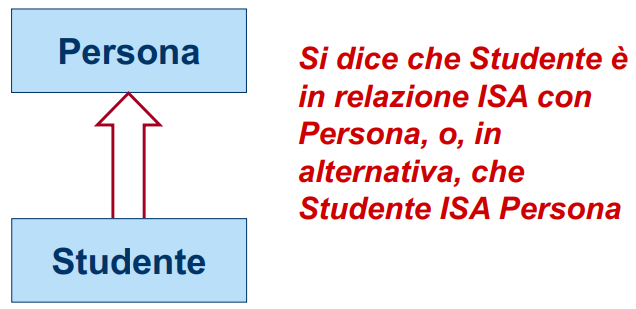
\includegraphics[width = 0.50\textwidth]{Images/36.PNG}
\end{center}
\subsubsection{Ereditarietà su entità}
La relazione IS-A implica il \textbf{principio di ereditarietà}: ongi proprietà dell'entità padre è anche una proprietà della sottoentità, e non si riporta esplicitamente nel diagramma.
L'entità figlia può avere ovviamente ulteriori proprietà.
\subsection{Generalizzazione tra entità}
Finora, abbiamo considerato la relazione IS-A che stabilisce che l'entità padre è più generale della sottoentità.
Talvolta, però, l'entità padre può generalizzare diverse sottoentità rispetto ad un unico criterio. In questo caso si parla di \textbf{generalizzazione}.
Nella generalizzazione, le sottoentità hanno insiemi di istanze disgiunti a coppie (anche se in alcune varianti del modello E-R, si può specificare se due sottoentità della stessa entità padre sono disgiunte o no).
Una generalizzazione può essere di due tipi:
\begin{itemize}
    \item \textbf{Completa}: l'unione delle istanze delle sottoentità è uguale all'insieme delle istanze dell'entità padre; si indica con una freccia annerita
    \item \textbf{Non completa}: si indica con una freccia non riempita
\end{itemize}
Alla generalizzazione si associa una coppia di lettere che indica come interpretare la generalizzazione.
La prima lettera indica il tipo di generalizzazione e può assumere i valori:
\begin{itemize}
    \item \textbf{t} per le generalizzazione complete (totali)
    \item \textbf{p} per le generalizzazioni non complete (parziali)
\end{itemize}
\newpage
\noindent
La seconda lettera invece indica se le sottoentità si sovrappongono o meno; essa può assumere i valori:
\begin{itemize}
    \item \textbf{e} se le sottoentità non si sovrappongono (esclusiva)
    \item \textbf{s} se le sottoentità si sovrappongono (sovrapposte)
\end{itemize}
\begin{center}
    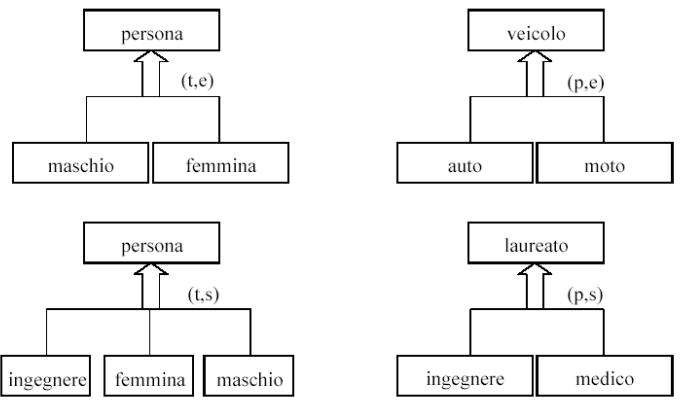
\includegraphics[width = 0.77\textwidth]{Images/37.PNG}
\end{center}
Nel modello E-R vige la regola che una entità può avere \textbf{al massimo una} entità padre. In altre parole, il modello E-R \textbf{non ammette ereditarietà multipla}.
Ovviamente, quando si contano i padri di una sottoentità si tiene conto anche di eventuali relazioni \textbf{IS-A} che essa ha con altre entità.
\begin{center}
    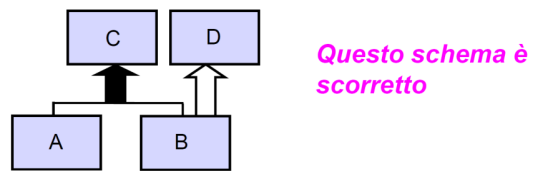
\includegraphics[width = 0.60\textwidth]{Images/38.PNG}
\end{center}
\subsubsection{Generalizzazioni ed ereditarietà}
Il \textbf{principio di ereditarietà} vale anche per le generalizzazioni: ogni proprietà dell'entità padre è anche una proprietà della sottoentità, e non si riporta esplicitamente nel diagramma.
L'entita figlia può avere ovviamente ulteriori proprietà.
\subsubsection{Diverse generalizzazioni della stessa classe}
La stessa entità può essere padre in diverse generalizzazioni.
Concettualmente, non c'è alcuna correlazione tra due generalizzazioni diverse, perché rispondono a due criteri diversi di classificare le istanze delle entità padre.
\subsubsection{Differenza tra due IS-A e una generalizazione}
Ci si potrebbe chiedere se non si possa utilizzare due IS-A per rappresentare una generalizzazione.
In realtà, le due (o più) sottoclassi che derivano da una generalizzazione derivano da uno stesso criterio di classificazione delle istanze della superclasse.
Le due sottoentità di due IS-A differenti invece sono indipendenti, nel senso che il loro significato non deriva dallo stesso criterio di classificazione delle istanze della entità padre.
\subsubsection{Altre proprietà}
Vi sono altre proprietà della generalizzazione:
\begin{itemize}
    \item Possono esistere gerarchie a più livelli e multiple generalizzazioni allo stesso livello
    \item Un'entità può essere inclusa in più gerarchie, come genitore e/o come figlia
    \item Se una generalizzazione ha solo un'entità figlia, si parla di \textbf{sottoinsieme}
\end{itemize}
\subsection{Relazione IS-A fra relazioni}
Nel caso di una relazione IS-A fra relazioni la semantica non cambia rispetto al caso della relazione IS-A tra entità:
se in uno schema $S$ è definita la relazione IS-A tra $R$ e $Q$ ($R$ IS-A $Q$, dove $R$ e $Q$ sono due relazioni con lo stesso grado e gli stessi ruoli), allora
in ogni istanza $I$ dello schema $S$, si ha che
$$istanze(I, R) \subseteq istanze(I, Q)$$
\begin{center}
    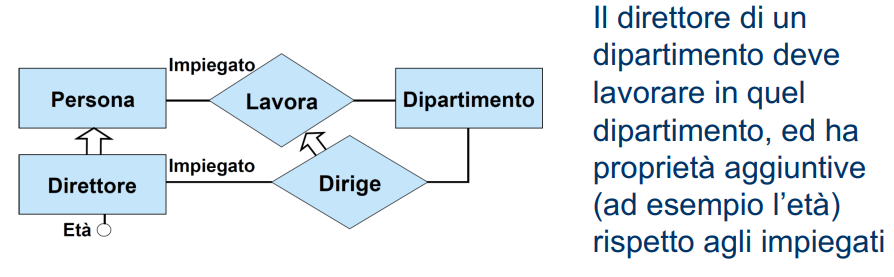
\includegraphics[width = 0.90\textwidth]{Images/39.PNG}
\end{center}
\subsection{Vincoli non esprimibili nel diagramma E-R}
Gli schemi E-R permettono di cogliere la maggior parte delle interrelazioni tra i dati del dominio d'interesse.
Tuttavia alcune interrelazioni non possono essere colte direttamente da uno schema E-R.
Talli interrelazioni vanno in ogni caso tenute presenti attraverso delle asserzioni aggiuntive dette \textbf{vincoli esterni al diagramma}, o semplicemente, \textbf{vincoli esterni}.
Come rappresentiamo tali vincoli?
\begin{itemize}
    \item Attraverso formalismi opportuni (es. \textbf{logica matematica})
    \item Attraverso asserzioni in linguaggio naturale (che devono essere il più possibile \textbf{precise e non ambigue})
\end{itemize}
\subsection{Documentazione associata agli schemi E-R}
Oltre al diagramma E-R, lo schema concettuale è descritto dal cosiddetto \textbf{dizionario dei dati}: esso è costituito dalle tabelle di
\begin{itemize}
    \item Entità
    \item Relazioni 
    \item Attributi 
    \item Vincoli esterni
\end{itemize}
\begin{center}
    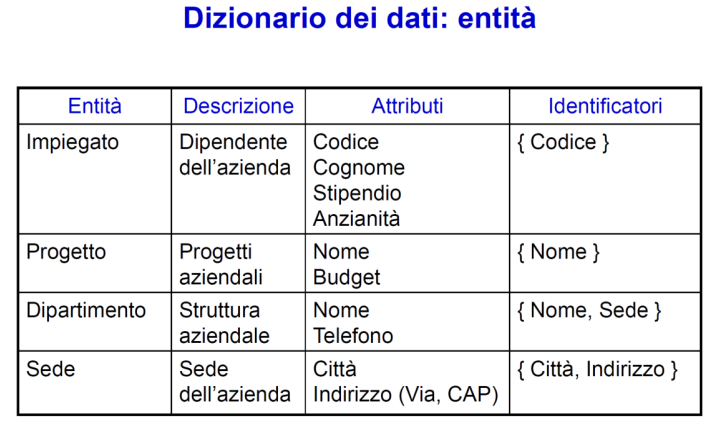
\includegraphics[width = 0.75\textwidth]{Images/40.PNG}
\end{center}
\begin{center}
    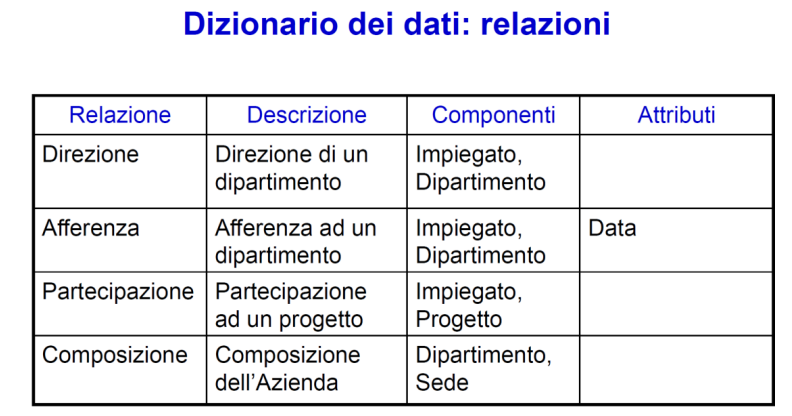
\includegraphics[width = 0.80\textwidth]{Images/41.PNG}
\end{center}
\begin{center}
    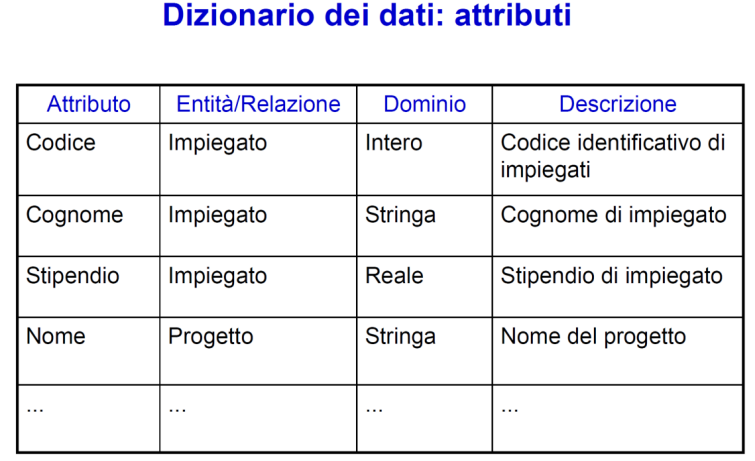
\includegraphics[width = 0.75\textwidth]{Images/42.PNG}
\end{center}
\begin{center}
    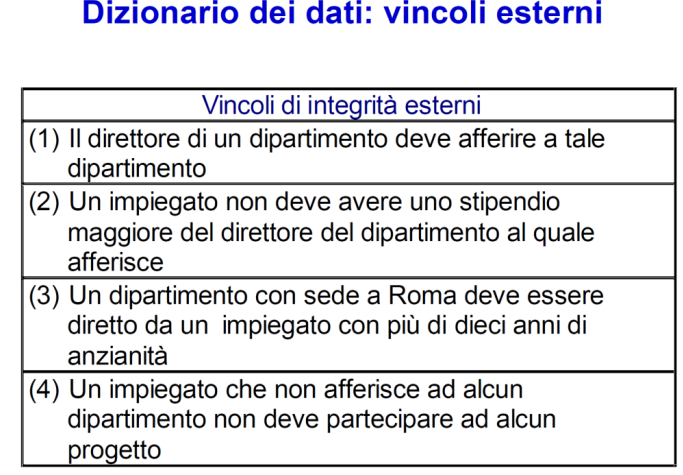
\includegraphics[width = 0.75\textwidth]{Images/43.PNG}
\end{center}
In particolare, il dizionario dei vincoli esterni può avere, a sua volta, altri vincoli esterni espressi in un altro dizionario.

\end{document}